\documentclass[12pt]{article}

% ---------- Packages ----------
\usepackage[a4paper,margin=2cm]{geometry}
\usepackage{amsmath}
\usepackage{siunitx}
\usepackage{tikz}
\usepackage[none]{hyphenat}
\usepackage{enumitem}
\usetikzlibrary{arrows.meta, calc}

% ---------- TikZ styles ----------
\tikzset{
    force/.style={->, thick},
    box/.style={draw, minimum width=2cm, minimum height=1cm}
}

% ---------- Document ----------
\begin{document}

\section*{Resultant Forces and Motion}

\begin{itemize}
    \item If forces are unbalanced, the resultant force $\neq \SI{0}{N}$ and the object undergoes acceleration.
    \item If forces are balanced, the resultant force $= \SI{0}{N}$ and the object moves at constant velocity.
\end{itemize}

\hrule
\vspace{0.8cm}

% ---------- Scenario 1 ----------
\noindent
\begin{minipage}[t]{0.48\textwidth}

\textbf{1. Car accelerates from rest}

\vspace{0.5cm}
$time = \SI{0}{s}$ \\
$mass = \SI{1200}{kg}$ \\
$velocity = \SI{0}{m/s}$ \\

\vspace{0.5cm}

\begin{center}
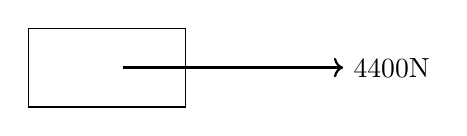
\begin{tikzpicture}

    % Box
    \node[box] (B) at (0,0) {};

    % Force
    \draw[force] ($(B.center)+(0.2,0)$) -- (3,0) node[right] {4400N};

\end{tikzpicture}
\end{center}

\end{minipage}
\hfill
\begin{minipage}[t]{0.48\textwidth}

\begin{itemize}[label={}, leftmargin=*]
    \item Calculate the resultant force acting on the car.

    \vspace{2.0cm}
    \[
    \makebox[\linewidth][r]{$F_{\text{resultant}} = \rule{3cm}{0.4pt}\ \text{N}$}
    \]

    \item Using Newton’s second law, $a = \dfrac{F}{m}$, determine the acceleration of the car.

    \vspace{2.0cm}
    \[
    \makebox[\linewidth][r]{$a = \rule{3cm}{0.4pt}\ \text{m/s}^{2}$}
    \]
\end{itemize}

\end{minipage}

\vspace{1.2cm}

% ---------- Scenario 2 ----------
\noindent
\begin{minipage}[t]{0.48\textwidth}

\textbf{2. Car accelerating}

\vspace{0.5cm}
$time = \SI{8}{s}$ \\
$mass = \SI{1200}{kg}$ \\
$velocity = \SI{24}{m/s}$ \\

\vspace{0.5cm}

\begin{center}
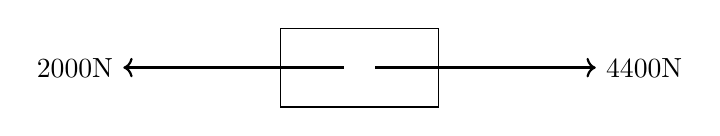
\begin{tikzpicture}

    % Box
    \node[box] (B) at (0,0) {};

    % Forces
    \draw[force] ($(B.center)+(0.2,0)$) -- (3,0) node[right] {4400N};
    \draw[force] ($(B.center)+(-0.2,0)$) -- (-3,0) node[left] {2000N};

\end{tikzpicture}
\end{center}

\end{minipage}
\hfill
\begin{minipage}[t]{0.48\textwidth}

\begin{itemize}[label={}, leftmargin=*]
    \item Calculate the resultant force acting on the car.

    \vspace{2.0cm}
    \[
    \makebox[\linewidth][r]{$F_{\text{resultant}} = \rule{3cm}{0.4pt}\ \text{N}$}
    \]

    \item Using Newton’s second law, $a = \dfrac{F}{m}$, determine the acceleration of the car.

    \vspace{2.0cm}
    \[
    \makebox[\linewidth][r]{$a = \rule{3cm}{0.4pt}\ \text{m/s}^{2}$}
    \]
\end{itemize}

\end{minipage}

\vspace{1.2cm}

% ---------- Scenario 3 ----------
\noindent
\begin{minipage}[t]{0.48\textwidth}

\textbf{3. Car accelerating}

\vspace{0.5cm}
$time = \SI{16}{s}$ \\
$mass = \SI{1200}{kg}$ \\
$velocity = \SI{35}{m/s}$ \\

\vspace{0.5cm}

\begin{center}
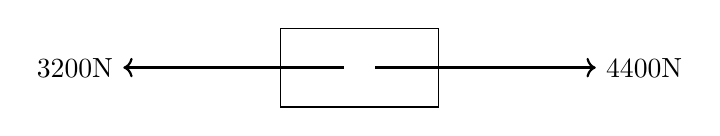
\begin{tikzpicture}

    % Box
    \node[box] (B) at (0,0) {};

    % Forces
    \draw[force] ($(B.center)+(0.2,0)$) -- (3,0) node[right] {4400N};
    \draw[force] ($(B.center)+(-0.2,0)$) -- (-3,0) node[left] {3200N};

\end{tikzpicture}
\end{center}

\end{minipage}
\hfill
\begin{minipage}[t]{0.48\textwidth}

\begin{itemize}[label={}, leftmargin=*]
    \item Calculate the resultant force acting on the car.

    \vspace{2.0cm}
    \[
    \makebox[\linewidth][r]{$F_{\text{resultant}} = \rule{3cm}{0.4pt}\ \text{N}$}
    \]

    \item Using Newton’s second law, $a = \dfrac{F}{m}$, determine the acceleration of the car.

    \vspace{2.0cm}
    \[
    \makebox[\linewidth][r]{$a = \rule{3cm}{0.4pt}\ \text{m/s}^{2}$}
    \]
\end{itemize}

\end{minipage}

\vspace{1.2cm}

% ---------- Scenario 4 ----------
\noindent
\begin{minipage}[t]{0.48\textwidth}

\textbf{4. Car at terminal velocity}

\vspace{0.5cm}
$time = \SI{24}{s}$ \\
$mass = \SI{1200}{kg}$ \\
$velocity = \SI{42}{m/s}$ \\

\vspace{0.5cm}

\begin{center}
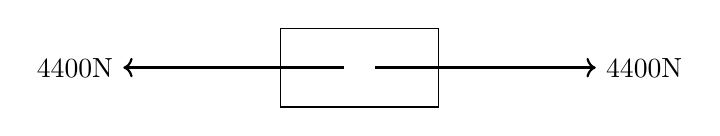
\begin{tikzpicture}

    % Box
    \node[box] (B) at (0,0) {};

    % Forces
    \draw[force] ($(B.center)+(0.2,0)$) -- (3,0) node[right] {4400N};
    \draw[force] ($(B.center)+(-0.2,0)$) -- (-3,0) node[left] {4400N};

\end{tikzpicture}
\end{center}

\end{minipage}
\hfill
\begin{minipage}[t]{0.48\textwidth}

\begin{itemize}[label={}, leftmargin=*]
    \item Calculate the resultant force acting on the car.

    \vspace{2.0cm}
    \[
    \makebox[\linewidth][r]{$F_{\text{resultant}} = \rule{3cm}{0.4pt}\ \text{N}$}
    \]

    \item Using Newton’s second law, $a = \dfrac{F}{m}$, determine the acceleration of the car.

    \vspace{2.0cm}
    \[
    \makebox[\linewidth][r]{$a = \rule{3cm}{0.4pt}\ \text{m/s}^{2}$}
    \]
\end{itemize}

\end{minipage}

\noindent
\begin{minipage}[t]{0.48\textwidth}

\textbf{1. Skydiver just after jumping}

\vspace{0.5cm}
$time = \SI{0}{s}$ \\
$mass = \SI{70}{kg}$ \\
$velocity = \SI{0}{m/s}$ \\

\vspace{0.5cm}

\begin{center}
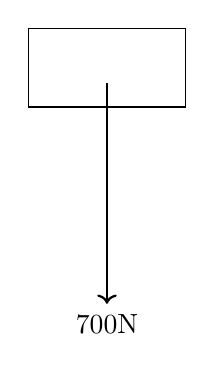
\begin{tikzpicture}

    % Box
    \node[box] (B) at (0,0) {};

    % Forces (vertical)
    \draw[force] ($(B.center)+(0,-0.2)$) -- (0,-3) node[below] {700N};
    % No air resistance yet (approximately)

\end{tikzpicture}
\end{center}

\end{minipage}
\hfill
\begin{minipage}[t]{0.48\textwidth}

\begin{itemize}[label={}, leftmargin=*]
    \item Calculate the resultant force acting on the skydiver.

    \vspace{2.0cm}
    \[
    \makebox[\linewidth][r]{$F_{\text{resultant}} = \rule{3cm}{0.4pt}\ \text{N}$}
    \]

    \item Using Newton’s second law, $a = \dfrac{F}{m}$, determine the acceleration of the skydiver.

    \vspace{2.0cm}
    \[
    \makebox[\linewidth][r]{$a = \rule{3cm}{0.4pt}\ \text{m/s}^{2}$}
    \]
\end{itemize}

\end{minipage}

\vspace{1.2cm}

% ---------- Scenario 2 ----------
\noindent
\begin{minipage}[t]{0.48\textwidth}

\textbf{2. Skydiver accelerating}

\vspace{0.5cm}
$time = \SI{6}{s}$ \\
$mass = \SI{70}{kg}$ \\
$velocity = \SI{25}{m/s}$ \\

\vspace{0.5cm}

\begin{center}
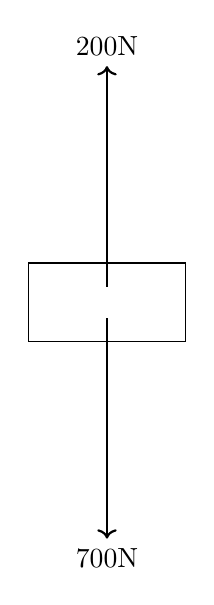
\begin{tikzpicture}

    % Box
    \node[box] (B) at (0,0) {};

    % Forces (vertical)
    \draw[force] ($(B.center)+(0,-0.2)$) -- (0,-3) node[below] {700N};
    \draw[force] ($(B.center)+(0,0.2)$) -- (0,3) node[above] {200N};

\end{tikzpicture}
\end{center}

\end{minipage}
\hfill
\begin{minipage}[t]{0.48\textwidth}

\begin{itemize}[label={}, leftmargin=*]
    \item Calculate the resultant force acting on the skydiver.

    \vspace{2.0cm}
    \[
    \makebox[\linewidth][r]{$F_{\text{resultant}} = \rule{3cm}{0.4pt}\ \text{N}$}
    \]

    \item Using Newton’s second law, $a = \dfrac{F}{m}$, determine the acceleration of the skydiver.

    \vspace{2.0cm}
    \[
    \makebox[\linewidth][r]{$a = \rule{3cm}{0.4pt}\ \text{m/s}^{2}$}
    \]
\end{itemize}

\end{minipage}

\vspace{1.2cm}

% ---------- Scenario 3 ----------
\noindent
\begin{minipage}[t]{0.48\textwidth}

\textbf{3. Skydiver accelerating (approaching terminal velocity)}

\vspace{0.5cm}
$time = \SI{12}{s}$ \\
$mass = \SI{70}{kg}$ \\
$velocity = \SI{45}{m/s}$ \\

\vspace{0.5cm}

\begin{center}
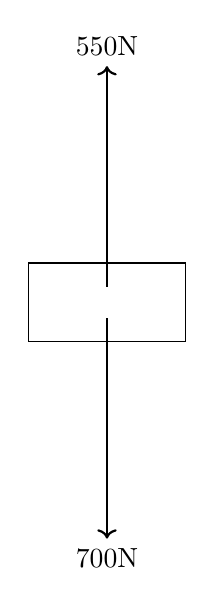
\begin{tikzpicture}

    % Box
    \node[box] (B) at (0,0) {};

    % Forces (vertical)
    \draw[force] ($(B.center)+(0,-0.2)$) -- (0,-3) node[below] {700N};
    \draw[force] ($(B.center)+(0,0.2)$) -- (0,3) node[above] {550N};

\end{tikzpicture}
\end{center}

\end{minipage}
\hfill
\begin{minipage}[t]{0.48\textwidth}

\begin{itemize}[label={}, leftmargin=*]
    \item Calculate the resultant force acting on the skydiver.

    \vspace{2.0cm}
    \[
    \makebox[\linewidth][r]{$F_{\text{resultant}} = \rule{3cm}{0.4pt}\ \text{N}$}
    \]

    \item Using Newton’s second law, $a = \dfrac{F}{m}$, determine the acceleration of the skydiver.

    \vspace{2.0cm}
    \[
    \makebox[\linewidth][r]{$a = \rule{3cm}{0.4pt}\ \text{m/s}^{2}$}
    \]
\end{itemize}

\end{minipage}

\vspace{1.2cm}

% ---------- Scenario 4 ----------
\noindent
\begin{minipage}[t]{0.48\textwidth}

\textbf{4. Skydiver at terminal velocity}

\vspace{0.5cm}
$time = \SI{18}{s}$ \\
$mass = \SI{70}{kg}$ \\
$velocity = \SI{55}{m/s}$ \\

\vspace{0.5cm}

\begin{center}
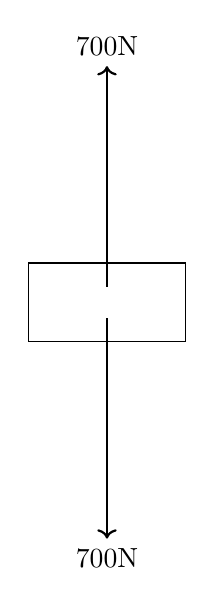
\begin{tikzpicture}

    % Box
    \node[box] (B) at (0,0) {};

    % Forces (vertical) - balanced
    \draw[force] ($(B.center)+(0,-0.2)$) -- (0,-3) node[below] {700N};
    \draw[force] ($(B.center)+(0,0.2)$) -- (0,3) node[above] {700N};

\end{tikzpicture}
\end{center}

\end{minipage}
\hfill
\begin{minipage}[t]{0.48\textwidth}

\begin{itemize}[label={}, leftmargin=*]
    \item Calculate the resultant force acting on the skydiver.

    \vspace{2.0cm}
    \[
    \makebox[\linewidth][r]{$F_{\text{resultant}} = \rule{3cm}{0.4pt}\ \text{N}$}
    \]

    \item Using Newton’s second law, $a = \dfrac{F}{m}$, determine the acceleration of the skydiver.

    \vspace{2.0cm}
    \[
    \makebox[\linewidth][r]{$a = \rule{3cm}{0.4pt}\ \text{m/s}^{2}$}
    \]
\end{itemize}

\end{minipage}

\end{document}
